\subsection{FRFs of the system due to a single point force}
\label{subsec:FRFs_of_the_system_due_to_a_single_point_force}

Once the FRFs function is defined, we can think of interrogate the structure to see how it reacts due to a single point force applied at a specific coordinate.

In particular, we can consider a sinusoidal force applied at coordinate $x_k = 0.9m$ and see how the structure reacts at a set of coordinates $x_j = [0.2 0.4 0.6 0.8 1.0 1.2]m$.
A graphical representation of the considered situation can be seen in Figure \ref{fig:beam_single_point_force}.

\begin{figure}[H]
    \centering
    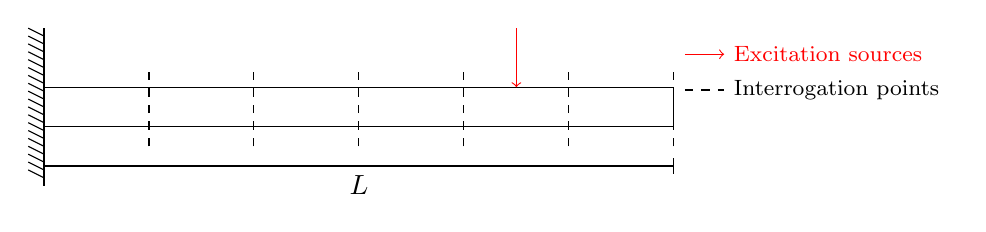
\begin{tikzpicture}[xscale=1, yscale=0.5]

        \draw (0,-0.5) rectangle (8, 0.5);
        \draw[|-|] (0, -1.5) -- (8, -1.5) node[midway, below]{$L$};

        \draw (0, -2) -- (0,  2);

        \foreach \y in {-1.8, -1.6, ..., 1.8}
        \draw (0, \y) -- ++(-0.2, +0.2);

        \foreach \x in {0.2, 0.4, ..., 1.2}
        \draw[dashed] (\x * 8/1.2, -1.0) -- ++(0.0, +2.0);

        \draw[<-, red] (0.9 * 8/1.2, 0.5) -- ++(0.0, +1.5);

        % Add legend
        \node [matrix, font = \footnotesize, below right, row sep = 0cm] at (current bounding box.north east)
        {
            \draw[->, red] (0, 0) -- ++(0.5, 0) node[right, red] {Excitation sources}; \\
            \draw[dashed, black] (0, 0) -- ++(0.5, 0) node[right, black] {Interrogation points}; \\
        };

    \end{tikzpicture}
    \caption{Analyzed situation: single input, multiple outputs}
    \label{fig:beam_single_point_force}
\end{figure}

Since we are now considering $6$ different coordinates, we will have $6$ different FRFs, each one describing the response of the structure at a specific coordinate due to the excitation $f(t) = F_0 \sin(\Omega t) = 1 \sin(\Omega t)$.

By doing so, we obtain the module and phase plots reported in Figure \ref{fig:FRFs_single_point_force}.

\begin{center}
    \huge{Plot to be replaced with the correct one.}
\end{center}

\begin{figure}[H]
    \centering
    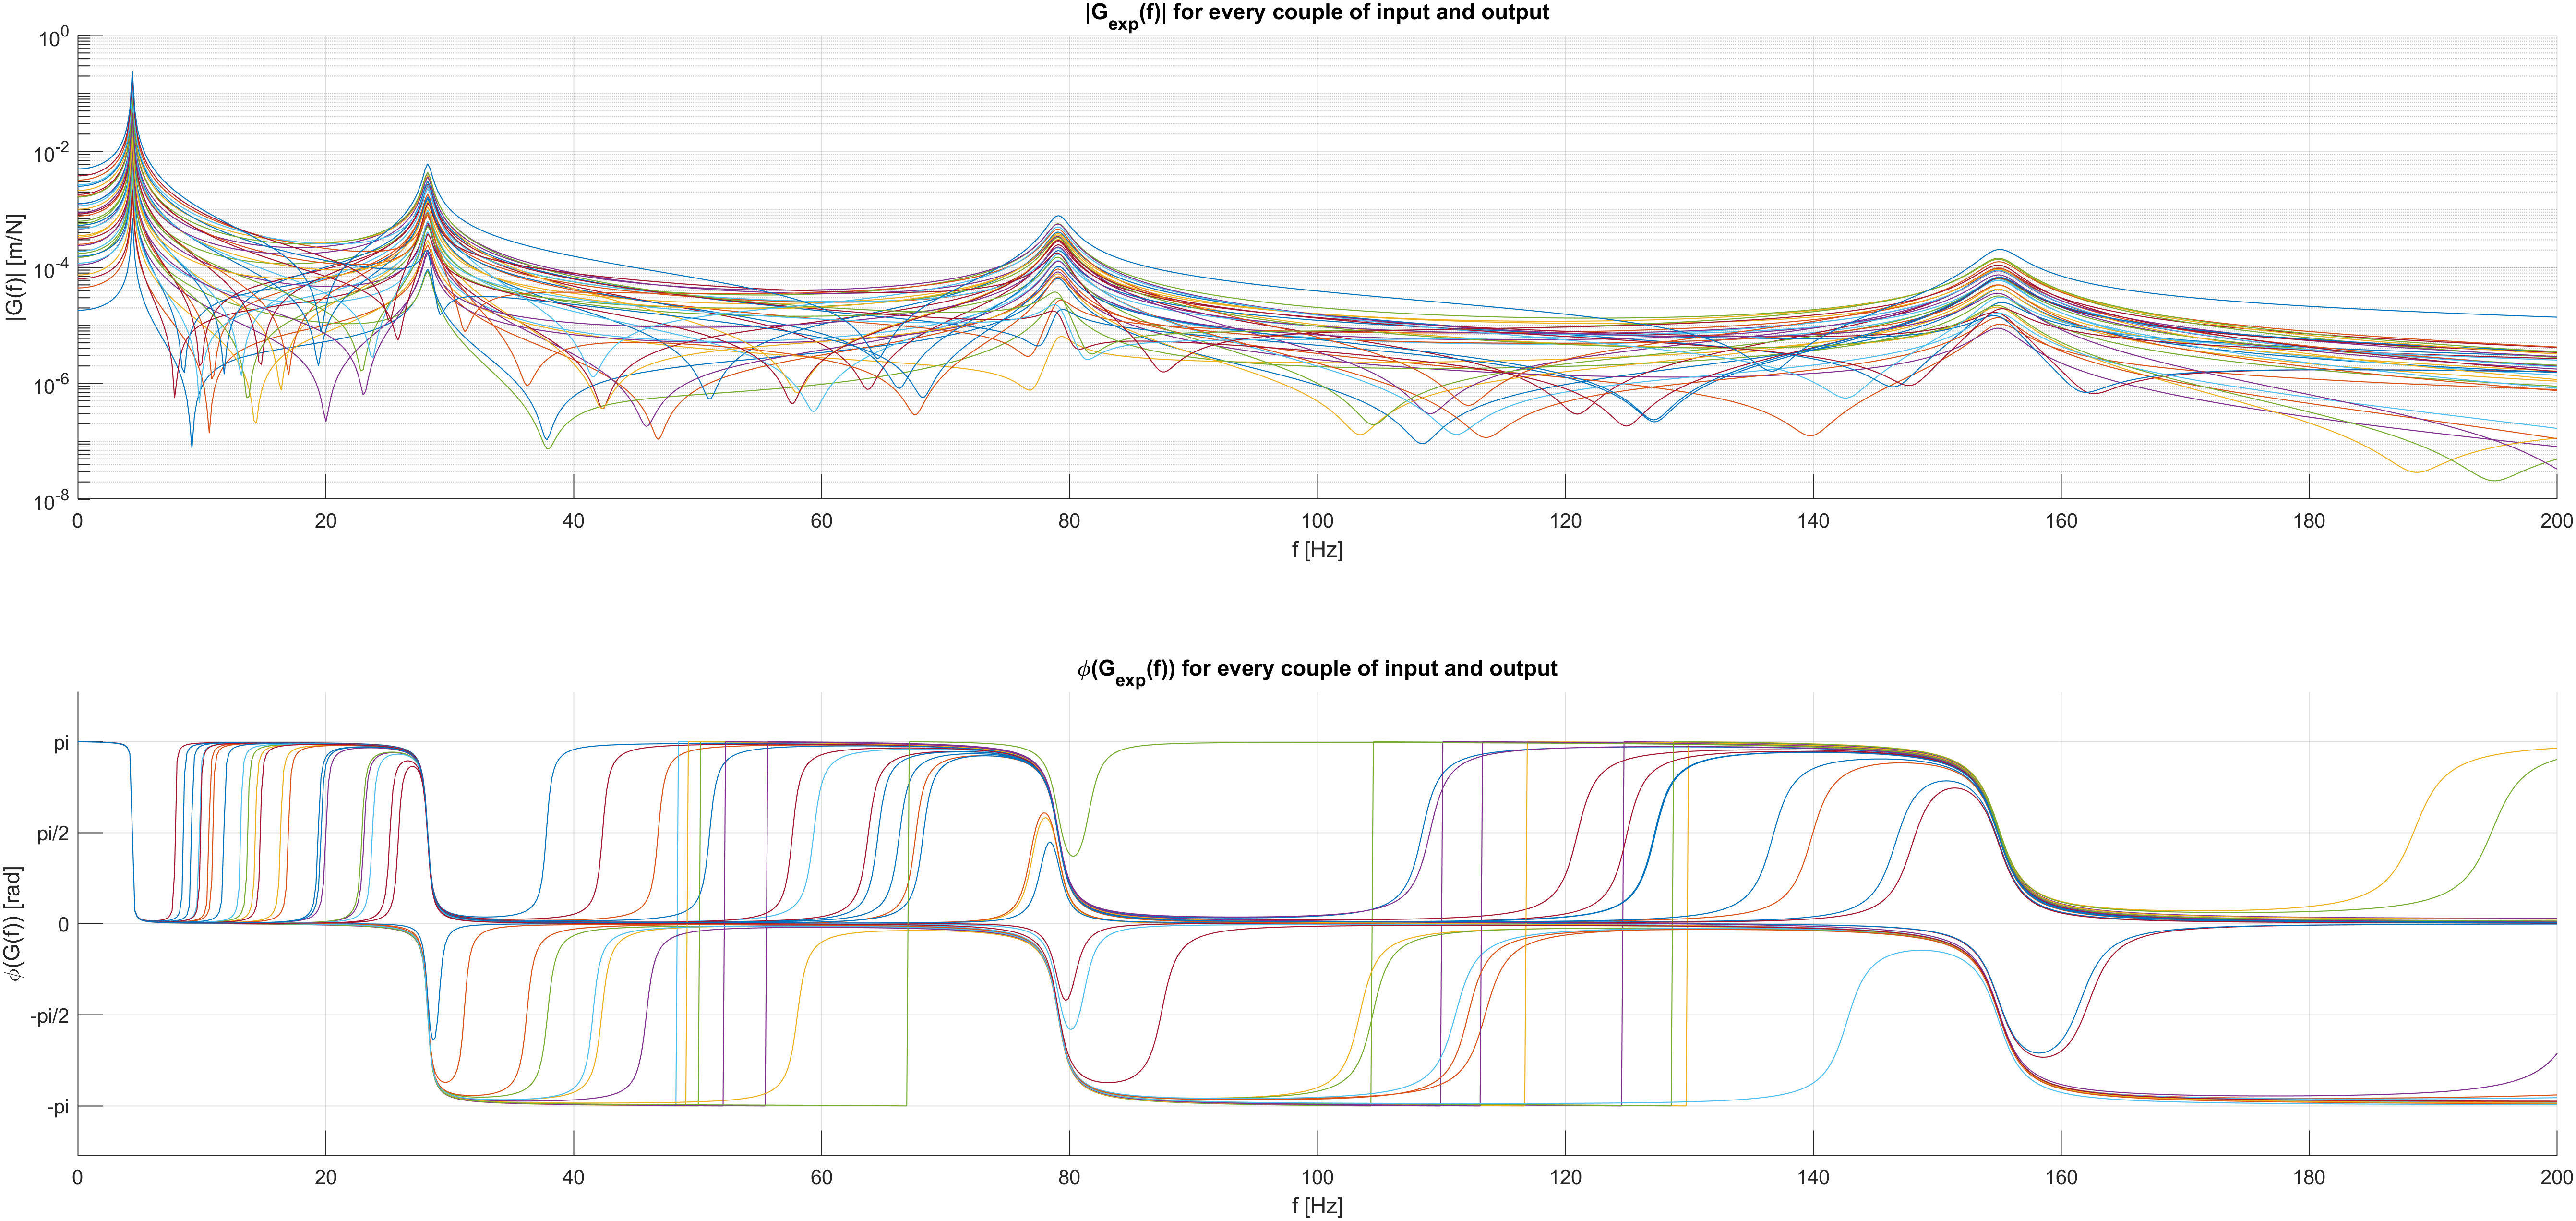
\includegraphics[width=\textwidth]{img/MATLAB/Part_A/Experimental_FRF_couple_all.png}
    \caption{FRFs of the system due to a single point force. Each color in the plot represents the FRF of the structure at a specific output coordinate.}
    \label{fig:FRFs_single_point_force}
\end{figure}
